The results obtained for the initially given code polynomials are presented in this section. By examining the result for the BSC on figure \ref{fig:givenRandomFigure}, it can be seen that the code with the highest code rate performs best. This is expected, since more redundancy is added. The constraint length does not appear to have a major influence on the performance in this channel, but it is hard to conclude anything when varying multiple parameters at once. Therefore, codes with fixed constraint length are compared in section \ref{sec:constantContraintLengthSection}.
For the burst simulations, it is seen in figure \ref{fig:givenBurstFigure} that Code 1 on average has significantly more errors in the message than the two other codes when comparing at the same burst length.
The result for the MBEC is more interesting. Here, the winner is less clear, and Code 1 and Code 2 perform equally well at low CER, while Code 2 performs best higher values. However, the code rate of Code 1 is only $1/2$ in contrast to the code rate of $1/3$ for Code 2, so it seems that the constraint length do have a big influence in this channel. This is investigated further in section  \ref{sec:constantCodeRateSection}.

\begin{figure}
\centering
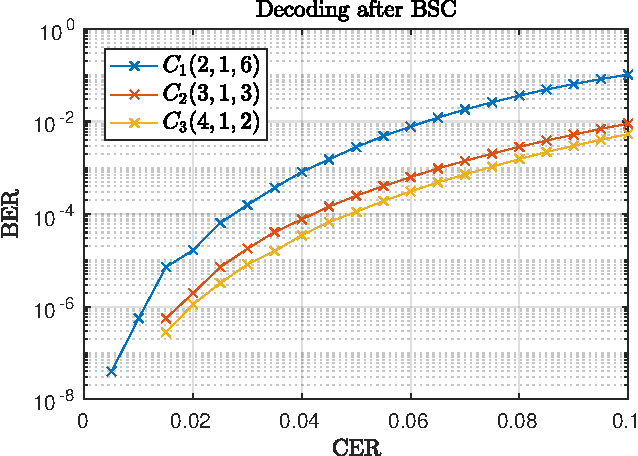
\includegraphics[scale=1]{../figures/qirandom.pdf} 
\caption{\textit{Comparison of given codes in BSC}\label{fig:givenRandomFigure}}
\end{figure}

\begin{figure}
\centering
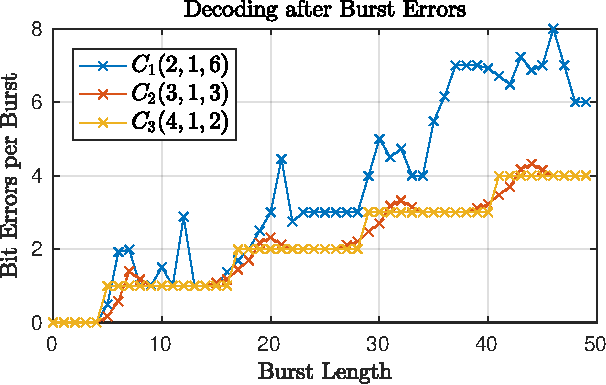
\includegraphics[scale=1]{../figures/qiburst.pdf} 
\caption{\textit{Comparison of given codes burst correction capabilities}\label{fig:givenBurstFigure}}
\end{figure}

\begin{figure}
\centering
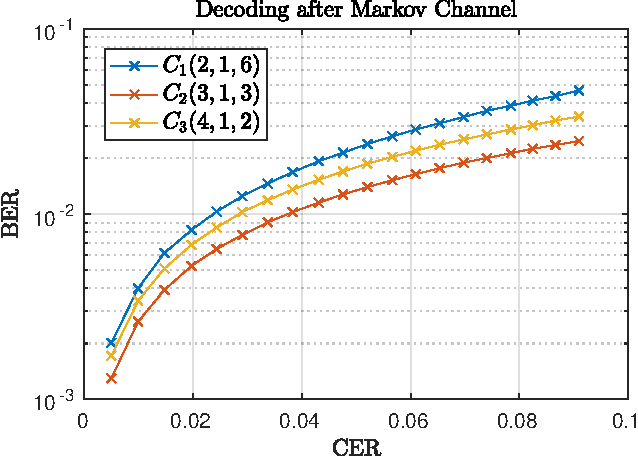
\includegraphics[scale=1]{../figures/qimarkov.pdf} 
\caption{\textit{Comparison of given codes in MBEC}\label{fig:givenMarkovFigure}}
\end{figure}
